%%%%%%%%%%%%%%%%%%%%%%%%%%%%%%%%%%%%%%%%%%%%%%%%%%%%%%%%%%%%%%%%%%%%%%
% Problem statement
\begin{statement}[
  problempoints=50,
  timelimit=1 sekunda,
  memorylimit=512 MiB,
]{Preokret}

\setlength\intextsep{-0.1cm}
\begin{wrapfigure}[6]{r}{0.2\textwidth}
\centering
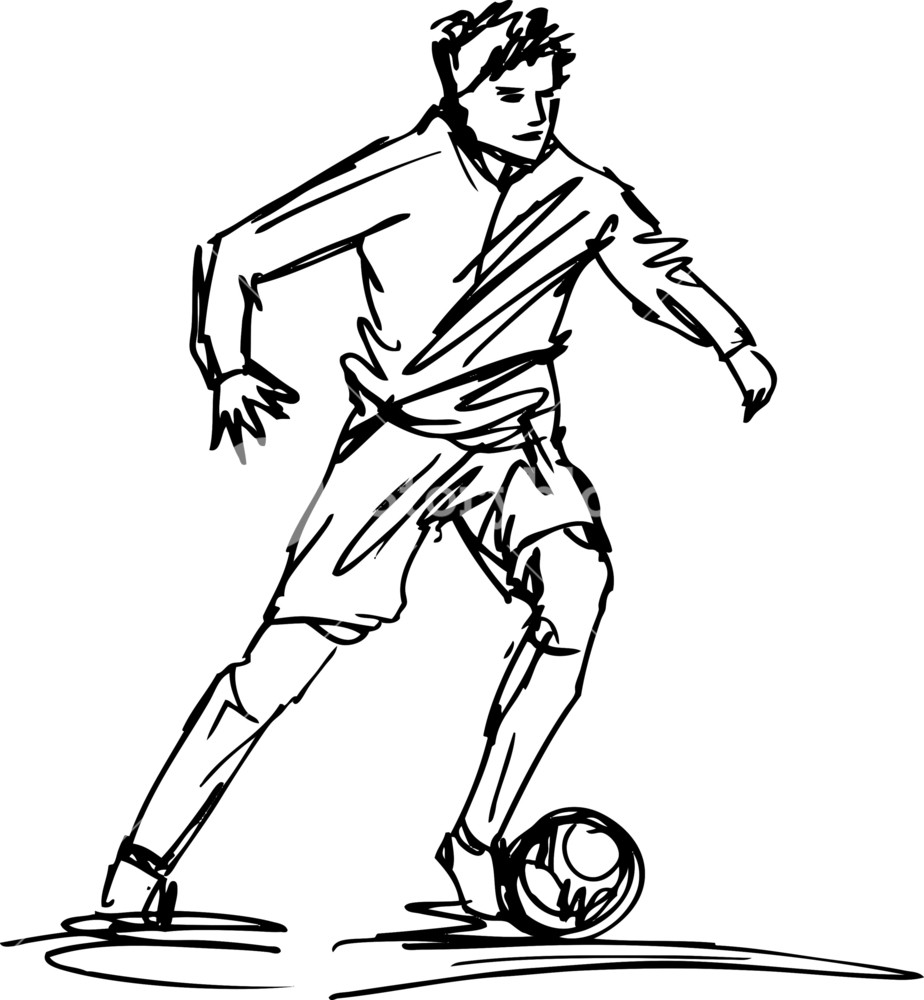
\includegraphics[width=0.2\textwidth]{img/fudbaler.jpg}
\end{wrapfigure}

  \textit{Štefanje} je, dan nakon Božića. U Engleskoj taj dan zovu \textit{Boxing day}. Dok kod nas
Štefanje tradicionalno prolazi u druženju s prijateljima i rješavanju
ostataka bogate blagdanske trpeze, u Engleskoj se više od stoljeća na taj dan
igra nogomet. Premiership, niže lige, amaterske lige -- svi igraju.

Pep je ovog Štefanja ostao doma. Kako je jučer malo pretjerao s francuskom
salatom i pečenjem činilo mu se logičnim dan provesti u krevetu, uz kutiju
Gastala, i ponovno odgledati i analizirati jedan stari meč svog Cityja s
nekim protivnikom.

Pep zna da je na utakmici postignuto ukupno $N$ golova i zna kojim su
redoslijedom timovi postizali te golove. Sada želi odgovoriti na tri pitanja:

\begin{enumerate}
  \item Kojim je rezultatom završila utakmica, tj. koliko je golova postigao
        City, a koliko protivnik?
  \item Koliko je različitih neriješenih rezultata bilo tijekom utakmice?
        Neriješenim rezultatom smatramo situaciju u kojoj oba tima imaju jednak
        broj postignutih golova. Početni rezultat \texttt{0:0} također se broji
        kao neriješen.
  \item Definirajmo \textit{preokret} tijekom utakmice kao situaciju u kojoj
        tim koji gubi, tj. ima strogo manje postignutih golova od drugog tima,
        postigne niz uzastopnih golova i nakon toga bude u vodstvu tj. ima strogo
        više postignutih golova od drugog tima. Pepa zanima koliki je bio najveći
        preokret na utakmici, tj. koji je bio najveći niz uzastopno postignutih
        golova takav da je klub prije početka niza gubio, a po završetku niza
        vodio? Na utakmici će sigurno biti barem jedan preokret.
\end{enumerate}


%%%%%%%%%%%%%%%%%%%%%%%%%%%%%%%%%%%%%%%%%%%%%%%%%%%%%%%%%%%%%%%%%%%%%%
% Input
\subsection*{Ulazni podaci}
U prvom je retku prirodan broj $N$ $(1 \le N \le 250)$ iz teksta zadatka.

U sljedećih se $N$ redaka nalazi po jedan broj $1$ ili $2$, oznake timova redom
kojim su postizali golove. City označimo brojem $1$, a protivnika brojem $2$.

%%%%%%%%%%%%%%%%%%%%%%%%%%%%%%%%%%%%%%%%%%%%%%%%%%%%%%%%%%%%%%%%%%%%%%
% Output
\subsection*{Izlazni podaci}
U prvi redak ispišite dva cijela broja odvojena razmakom, broj golova koje je
postigao City i broj golova koje je postigao protivnik.

U drugi redak ispišite prirodan broj, broj različitih neriješenih rezultata iz
teksta zadatka.

U treći redak ispišite cijeli broj, najveći preokret iz teksta zadatka.

%%%%%%%%%%%%%%%%%%%%%%%%%%%%%%%%%%%%%%%%%%%%%%%%%%%%%%%%%%%%%%%%%%%%%%
% Scoring
\subsection*{Bodovanje}
Točan ispis prvog retka vrijedi $1$ bod, točan ispis drugog $1$ bod, a točan
ispis trećeg retka vrijedi $3$ boda za svaki test podatak.

%%%%%%%%%%%%%%%%%%%%%%%%%%%%%%%%%%%%%%%%%%%%%%%%%%%%%%%%%%%%%%%%%%%%%%
% Examples
\subsection*{Probni primjeri}
\begin{tabularx}{\textwidth}{X'X'X}
\sampleinputs{test/preokret.dummy.in.1}{test/preokret.dummy.out.1} &
\sampleinputs{test/preokret.dummy.in.2}{test/preokret.dummy.out.2} &
\sampleinputs{test/preokret.dummy.in.3}{test/preokret.dummy.out.3}
\end{tabularx}

\textbf{Pojašnjenje prvog probnog primjera:}
Rezultat utakmice kretao se na sljedeći način: \texttt{0:0}, \texttt{1:0},
\texttt{2:0}, \texttt{2:1}, \texttt{2:2}, \texttt{2:3}.  Ukupno su bila dva
različita neriješena rezultata: \texttt{0:0} i \texttt{2:2}. Najveći preokret
dogodio se kada je protivnik pri rezultatu \texttt{2:0} gubio te nizom od tri
uzastopna gola na kraju vodio \texttt{2:3}.

\textbf{Pojašnjenje drugog probnog primjera:}
Rezultat utakmice kretao se na sljedeći način: \texttt{0:0}, \texttt{1:0},
\texttt{1:1}, \texttt{1:2}, \texttt{2:2}, \texttt{3:2}, \texttt{4:2},
\texttt{4:3}, \texttt{5:3}, \texttt{6:3}. Ukupno su bila tri različita
neriješena rezultata: \texttt{0:0}, \texttt{1:1}, \texttt{2:2}. Najveći
preokret dogodio se kada je City pri rezultatu \texttt{1:2} gubio te nizom od
tri uzastopna gola na kraju vodio rezultatom \texttt{4:2}.

%%%%%%%%%%%%%%%%%%%%%%%%%%%%%%%%%%%%%%%%%%%%%%%%%%%%%%%%%%%%%%%%%%%%%%
% We're done
\end{statement}

%%% Local Variables:
%%% mode: latex
%%% mode: flyspell
%%% ispell-local-dictionary: "croatian"
%%% TeX-master: "../hio.tex"
%%% End:
